\begin{center}
\tikzset{tbox/.style={draw, text badly centered, very thick, black, rectangle, inner sep=0, minimum width = 2.0 cm, minimum height = 1.0 cm}}
\tikzstyle{line} = [draw, -latex', thick]
\begin{tikzpicture}[x=1cm,y=1cm, text badly centered]
%\pgfresetboundingbox
\draw[use as bounding box, anchor = north west,draw=none] (-5.5,-3.25) rectangle (5.5,3.25);
\clip (-5.5,-3.25) rectangle (5.5,3.25);
\visible<2->{\node[anchor=west, text width=2 cm] (obs) at (-5.0,0) {observation \only<8->{$x^{*}\in\mathbb{R}^{d}$} };}
\visible<7->{\node [tbox,minimum width=2.0 cm, text width = 2.0 cm] (model) at (0,0) {model};}
\visible<2->{\node[anchor=east, text width=2 cm] (preds) at (5.0,0) {property \only<8->{$y\in\mathbb{R}$}};}
\visible<4->{\node[circle,minimum size=5cm, fill=orange, opacity=0.15,text opacity=1.0] at (0,0){};}
\visible<4->{\node[text width=2.5 cm, text badly centered]  at (0,1.75){model family \only<8->{$\mathcal{T}$ maps $\mathcal{R}^{d}\rightarrow \mathbb{R}$}};}
\visible<7->{\node[text width=2.5 cm] (params) at (0,-1.75){parameters \only<8->{$w\in\mathbb{R}^{p}$}};}
%% paths
\visible<7->{\path[draw,very thick,->] (obs) -- (model);}
\visible<7->{\path[draw,very thick,->] (model) -- (preds);}
\visible<7->{\path[draw,very thick,->] (params) -- (model);}
\def \cssize {1.0 cm}
\def \psize {1.15 cm}
%\visible<7->{\node at(0,0) {
\includegraphics[width=5cm]{images-top/ml-or-regression}};}
\visible<3-6>{
{\node[circle,draw, thick, minimum width =\cssize,path picture={\node at (path picture bounding box.center){
\includegraphics[width= \psize]{satistical_learning/images/m1}}; }] (m1) at (-4.0,-2.5){};}
{\node[circle,draw, thick, minimum width = \cssize,path picture={\node at (path picture bounding box.center){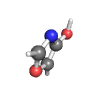
\includegraphics[width= \psize]{satistical_learning/images/m2}}; }] (m2) at (-3,-2.5){};}
{\node[circle,draw, thick, minimum width = \cssize,path picture={\node at (path picture bounding box.center){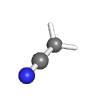
\includegraphics[width= \psize]{satistical_learning/images/m3}}; }] (m3) at (-4.0,-1.5){};}
{\node[circle,draw, thick, minimum width = \cssize,path picture={\node at (path picture bounding box.center){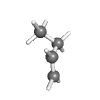
\includegraphics[width= \psize]{satistical_learning/images/m4}}; }] (m4) at (-3.0,-1.5){};}
{\node[circle,draw, thick, minimum width = \cssize,path picture={\node at (path picture bounding box.center){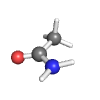
\includegraphics[width= \psize]{satistical_learning/images/m5}}; }] (m5) at (-2,-2.5){};}
{\node[circle,draw, thick, minimum width = \cssize,path picture={\node at (path picture bounding box.center){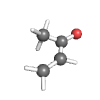
\includegraphics[width= \psize]{satistical_learning/images/m6}}; }] (m6) at (-2,-1.5){};}
{\node[circle,draw, thick, minimum width = \cssize,path picture={\node at (path picture bounding box.center){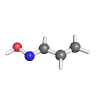
\includegraphics[width= \psize]{satistical_learning/images/m7}}; }] (m7) at (-5,-1.5){};}
{\node[circle,draw, thick, minimum width = \cssize,path picture={\node at (path picture bounding box.center){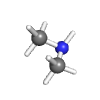
\includegraphics[width= \psize]{satistical_learning/images/m8}}; }] (m8) at (-5,-2.5){};}
}
\visible<3-6>{
{\node[anchor=east, text width=2 cm] (predsl) at (5.0,-2.0) {energy, structre...};}
}
\visible<5-6>{
\def\nudg{0.25}
\node (ds) at (-1,-2+\nudg){};
\node (dsy) at (-1,0.0+\nudg){};
\node (dsx) at (1.0,-2+\nudg){};
\node (xlab) at (0,-2.25+\nudg) {\large x};
\node (ylab) at (-1.25,-1+\nudg) {\large y};
\visible<1->{\path[line, thick] (ds.center) -- (dsx);}
\visible<1->{\path[line, thick] (ds.center) -- (dsy);}

\visible<1->{\path[line,thick,red] (-1,-0.85+\nudg) -- (1.0,-1.35+\nudg);}
\visible<1->{\path[line,thick,blue] (-1,-1.75+\nudg) -- (1.0,-0.5+\nudg);}
\visible<1->{\path[line,thick,purple] (-1,-0.75+\nudg) -- (1.0,-0.15+\nudg);}
}
\visible<6>{\path[line,thick,black] (m5.east) -| (xlab.south);}
\visible<6>{\path[line,thick,blue] (1.15,-0.5+\nudg) -| (predsl.north);}
\end{tikzpicture}
\end{center}